\chapter{HDMI}\label{chap:chap3}

Este capítulo descreve o trabalho realizado para cumprir a primeira parte do projeto: obter uma conexão HDMI entre recetor e transmissor. São descritas as várias configurações das placas HDMI disponíveis e ainda as arquiteturas desenvolvidas e implementadas para cumprir esta parte do projeto. 

\section{\textit{Hardware} utilizado} \label{sec:hardware}

Tal como mencionado no sub-capítulo \ref{sec:HDMIinFPGA}, para receber os dados provenientes do cabo HDMI e fazer a sua seleção são utilizadas duas placas HDMI (TB-FMCH-HDMI2 RX E TB-FMCH-HDMI2 TX) que, através das suas entradas e saída FMC de alta velocidade, conseguem enviar para e receber da FPGA os sinais de imagem e som. Nas imagens \ref{fig:rx} e \ref{fig:tx} é possível visualizar o recetor (TB-FMCH-HDMI2 RX) e o transmissor (TB-FMCH-HDMI2 TX) HDMI utilizados neste projeto. Em conjunto, estas duas placas são designadas apenas por TB-FMCH-HDMI2. Estas mesmas placas são constituídas por conectores HDMI onde é recebido o sinal HDMI que de seguida é enviado para um recetor ou transmissor, ADV7612 no caso do recetor e ADV7511 no caso do transmissor. Finalmente os sinais provenientes do recetor/transmissor são enviados para uma FGPA embebida na placa (XC6SLX45-3FGG484C) que, consoante a sua configuração, envia pelos conectores FMC os sinais de áudio e vídeo


\begin{figure}[h!]
	\begin{center}
		\leavevmode
		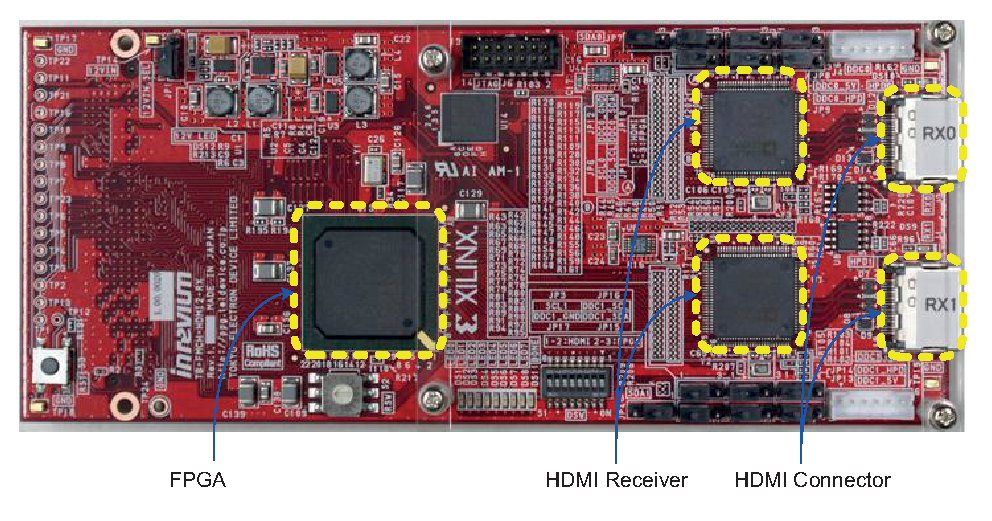
\includegraphics[width=1.0\textwidth]{placa_HDMI_rx_vet}
		\caption{TB-FMCH-HDMI2 RX, retirada de \cite{R009}}
		\label{fig:rx}
	\end{center}
\end{figure}

\begin{figure}[h!]
	\begin{center}
		\leavevmode
		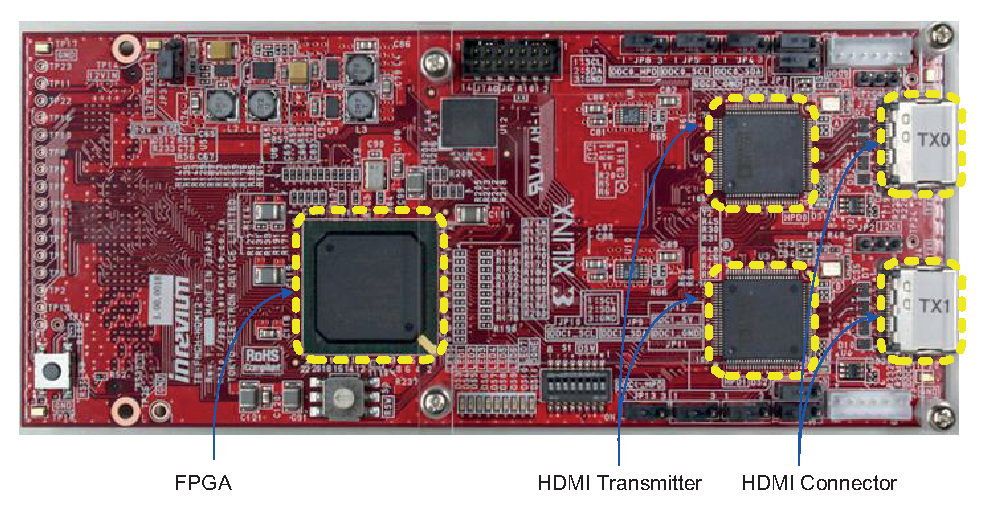
\includegraphics[width=1.0\textwidth]{placa_HDMI_tx_vet}
		\caption{TB-FMCH-HDMI2 TX, retirada de \cite{R009}}
		\label{fig:tx}
	\end{center}
\end{figure}
As placas possuem ainda uma PROM (\textit{Programmable read-only memory}) XCF16PFSG48C de configuração reprogramável que permite armazenar o \textit{bitstream} que configura a FPGA embebida do modo que se pretende. É esta FPGA embebida que em cada placa (RX e TX) é responsável pela seleção e envio ou receção dos dados pretendidos para ou dos conectores FMC, e como tal é necessário que estejam configuradas para realizarem tais procedimentos. O recurso a estas memórias reconfiguráveis vem permitir uma fácil alteração da configuração da FPGA uma vez que, segundo \cite{R026}, estas memórias de leitura permitem não só armazenar os \textit{bitstreams} de configuração da FPGA, mas também reconfigurá-los, caso se pretenda, de uma forma fácil e eficiente.

As reconfigurações destas memórias são realizadas através de um programador JTAG e ainda recorrendo a um \textit{software}. O \textit{software} utilizado neste projeto tem o nome de \textit{imPACT} e é disponibilizado pela \textit{Xilinx}. Após a conexão do conector JTAG à respectiva placa e ao computador (através de uma porta USB) é necessário inicializar o \textit{software} e programar a memória com o respetivo ficheiro pretendido. Em \cite{R025} são detalhadas informações acerca do programador utilizado e ainda sobre o procedimento para se reconfigurar as memórias. As reconfigurações realizadas neste projeto basearam-se nesse documento.

\subsection{Configurações da FPGA} \label{subsec:HDMIconfig}

A FPGA \textit{Spartan-6} (XC6SLX45-3FGG484C) embebida nas placas tem 3 configurações disponíveis. Estas variam não só no suporte que possuem, que pode ser apenas de imagem mas também de áudio, mas variam também no número de bits por imagem que estas podem ter. Nas secções seguintes serão brevemente abordadas as configurações disponíveis e como se pode tirar partido das mesmas no projeto que foi desenvolvido.

\subsubsection{Configuração por \textit{default}} \label{subsubsec:HDMIconfigdefault}

Esta configuração vem previamente escrita na memória PROM de fábrica e acaba por ser a mais simples de todas. Os dados enviados pelos conectores FMC são apenas referentes aos dados de imagem. As tabela \ref{table:HDMIdataRX} e \ref{table:HDMIdataTX} nas páginas \pageref{table:HDMIdataRX} e \pageref{table:HDMIdataTX} respectivamente identificam as portas às quais são atribuídas os sinais de dados de imagem HDMI tanto na placa recetora como na transmissora.

Esta configuração suporta a transmissão de imagens RGB (\textit{Red Green Blue}) com 10 bits. Assim sendo, tal como referido em \cite{R009}, independentemente da formatação das imagens da fonte HDMI o recetor ADV7612 integrado na placa recetora HDMI converte a imagem para o formato RGB e transmite de maneira a enviar os dados em apenas 10 bits. A tabela \ref{table:HDMIdefaultSimplified} da página \pageref{table:HDMIdefaultSimplified}, adaptada de \cite{R009}, apresenta brevemente quais as portas das placas utilizadas e que sinais são transmitidos nas mesmas, no entanto é possível encontrar na tabela \ref{table:HDMIdataDefaultdetail} do anexo \ref{ap1:HDMI} mais detalhes relativamente a estes dados. Os nomes dos sinais são referentes aos sinais em TB-FMCH-HDMI2 (tanto TX como RX), e como tal quando se faz referência à FPGA nestas tabelas estas correspondem às que estão embebidas nas placas HDMI. 

\begin{table}[h!]
	\centering
	\begin{tabular}{|c|c|c|c|}
		\hline
		\textbf{PIN}                                                                     & \textbf{FPGA -> FMC (RX)}                                                  & \textbf{FMC -> (TX)}                                                    & \textbf{Descrição}                                                      \\ \hline
		CLK0\_M2C\_P                                                                     & RX\#O\_LLC                                                                            & TX\#O\_DCLK                                                                           & \begin{tabular}[c]{@{}c@{}}Sinal de relógio dos\\   pixeis\end{tabular} \\ \hline
		LA00\_P\_CC                                                                      & RX\#0\_VSYNC                                                                          & TX\#0\_VSYNC                                                                          & \begin{tabular}[c]{@{}c@{}}Sincronização\\   Vertical\end{tabular}      \\ \hline
		LA01\_P\_CC                                                                      & RX\#0\_HSYNC                                                                          & TX\#0\_HSYNC                                                                          & \begin{tabular}[c]{@{}c@{}}Sincronização\\   Horizontal\end{tabular}    \\ \hline
		LA02\_P                                                                          & RX\#0\_DE                                                                             & TX\#0\_DE                                                                             & \begin{tabular}[c]{@{}c@{}}Sinal de \\ dados ativos\end{tabular}        \\ \hline
		\multirow{3}{*}{\begin{tabular}[c]{@{}c@{}}LA03\_P \\ a \\ LA32\_P\end{tabular}} & \multirow{3}{*}{\begin{tabular}[c]{@{}c@{}}RX\#0\_P0 \\ a \\ RX\#0\_P29\end{tabular}} & \multirow{3}{*}{\begin{tabular}[c]{@{}c@{}}TX\#0\_D0 \\ a \\ TX\#0\_D29\end{tabular}} & \multirow{3}{*}{Pixel de Imagem}                                        \\
		&                                                                                       &                                                                                       &                                                                         \\
		&                                                                                       &                                                                                       &                                                                         \\ \hline
	\end{tabular}
	\caption{Descrição e localização dos pinos de TB-FMCH-HDMI2 configurada por \textit{default}}
	\label{table:HDMIdefaultSimplified}
\end{table}

É de notar ainda que esta configuração é capaz de suportar até dois canais (RX0 e TX0, RX1 e TX1), no entanto nesta tabela apenas são apresentados os dados correspondentes ao canal 0 pois apenas será necessário utilizar um canal neste projeto. 

Apesar de ser um configuração simples, uma vez que apenas são transmitidos sinais de imagem em formato RGB, é uma configuração que será utilizada numa fase inicial em algumas arquiteturas implementadas que serão descritas na secção \ref{sec:HDMIarquiteturas}.

\subsubsection{Suporte de um canal de imagem e áudio} \label {subsubsec:HDMIconfig+audio}

Para além da configuração descrita anteriormente em \ref{subsubsec:HDMIconfigdefault} que apenas suporta a transmissão de imagem, existe ainda uma configuração capaz de suportar não só a transmissão de imagem mas também de som. A configuração que é escrita na PROM da placa recetora para programar a FPGA embebida controla o recetor ADV7612 de maneira a conseguir transmitir imagens no formato YCbCr ou RGB com 12 bits e também fazer a transmissão do audio em formato $I^{2}$S. O mesmo acontece na placa transmissora mas para ser capaz de receber estas configurações.

Assim como referido em \cite{R014}, neste caso a configuração da imagem está dependente da fonte HDMI, e é transmitida pelas placas tal como é emitida pela fonte, por outras palavras, se a fonte HDMI transmitir uma imagem em formato RGB é nesse mesmo que chega ao destino, no entanto se for transmitida uma imagem no formato YCbCr é nesse que chega ao seu destino. No caso do som, este é sempre transmitido em formato $I^{2}$S, o que implica a transmissão dos dados de áudio mas também sinais de relógio necessários à sua transmissão.

Na tabela \ref{table:HDMIaudiosuportSimplified} na página \pageref{table:HDMIaudiosuportSimplified} são brevemente apresentados as portas e os sinais usados com este tipo de configuração da FPGA embebida. Na tabela \ref{table:HDMI1canal+audioDETAIL} no anexo \ref{ap1:HDMI} é apresentada uma tabela semelhante a esta, mas que inclui mais detalhes relativamente aos pinos usados e ao seu uso. Ambas as tabelas foram adaptadas de \cite{R014} onde são apresentados todos os detalhes dos conectores FMC das placas.

\begin{table}[h!]
	\centering
	\begin{tabular}{|c|c|c|c|}
		\hline
		\textbf{PIN}                                                                           & \textbf{FPGA -\textgreater FMC (RX)}                                                 &\textbf{FMC -> FPGA (TX)}& \textbf{FPGA->HDMI\_TX} \\ \hline
		CLK0\_M2C\_P                                                                           & RX\#0\_LLC                                                                           & TX\#0\_DCLK                                                                          & \begin{tabular}[c]{@{}c@{}}Sinal de relógio dos\\ pixeis\end{tabular}                        \\ \hline
		LA00\_P\_CC                                                                            & RX\#0\_VSYNC                                                                         & TX\#0\_VSYNC                                                                         & Sincronização vertical                                                                       \\ \hline
		LA01\_P\_CC                                                                            & RX\#0\_HSYNC                                                                         & TX\#0\_HSYNC                                                                         & Sincronização horizontal                                                                     \\ \hline
		LA02\_P                                                                                & RX\#0\_DE                                                                            & TX\#0\_DE                                                                            & Sinal de dados ativos                                                                        \\ \hline
		\multirow{3}{*}{\begin{tabular}[c]{@{}c@{}}LA03\_P\\   a LA32\_P\end{tabular}}         & \multirow{3}{*}{RX\#0\_P0 a RX\#0\_P29}                                              & \multirow{3}{*}{TX\#0\_D0 a TX\#0\_D29}                                              & \multirow{3}{*}{\begin{tabular}[c]{@{}c@{}}Pixel de imagem do bit\\   0 ao 29\end{tabular}}  \\
		&                                                                                      &                                                                                      &                                                                                              \\
		&                                                                                      &                                                                                      &                                                                                              \\ \hline
		\multirow{2}{*}{\begin{tabular}[c]{@{}c@{}}LA00\_N\_CC\\   a LA01\_N\_CC\end{tabular}} & \multirow{2}{*}{RX\#0\_InputVideoStatus}                                             & \multirow{2}{*}{TX\#0\_InputVideoStatus}                                             & \multirow{2}{*}{\begin{tabular}[c]{@{}c@{}}Formato de video\\   (2D/3D)\end{tabular}}        \\
		&                                                                                      &                                                                                      &                                                                                              \\ \hline
		LA19\_N                                                                                & RX\#0\_MCLK                                                                          & TX\#0\_MCLK                                                                          & \textit{Master Clock} de som                                                                          \\ \hline
		LA20\_N                                                                                & RX\#0\_SCLK                                                                          & TX\#0\_SCLK                                                                          & \textit{Serial Clock} de som                                                                          \\ \hline
		\multirow{2}{*}{\begin{tabular}[c]{@{}c@{}}LA21\_N\\   a LA26\_N\end{tabular}}         & \multirow{2}{*}{RX\#0\_AP0 a RX\#0\_AP5}                                             & \multirow{2}{*}{TX\#0\_AP0 a TX\#0\_AP5}                                             & \multirow{2}{*}{Dados de som}                                                                \\
		&                                                                                      &                                                                                      &                                                                                              \\ \hline
		\multirow{2}{*}{\begin{tabular}[c]{@{}c@{}}LA27\_N\\   a LA32\_N\end{tabular}}         & \multirow{2}{*}{\begin{tabular}[c]{@{}c@{}}RX\#0\_P30 a\\   RX\#0\_P35\end{tabular}} & \multirow{2}{*}{\begin{tabular}[c]{@{}c@{}}TX\#0\_P30 a\\   TX\#0\_P35\end{tabular}} & \multirow{2}{*}{\begin{tabular}[c]{@{}c@{}}Pixel de imagem do bit\\   30 ao 35\end{tabular}} \\
		&                                                                                      &                                                                                      &                                                                                              \\ \hline
	\end{tabular}
	\centering
	\caption{Descrição e localização dos pinos de TB-FMCH-HDMI2 configurada para um canal de imagem e áudio}
	\label{table:HDMIaudiosuportSimplified}
\end{table}

Os dados referentes ao som transmitidos pela placa recetora e recebidos de seguida pela placa emissora estão mencionados com mais detalhe na tabela \ref{table:HDMI1canal+audioDETAIL} do anexo \ref{ap1:HDMI}, e tal como indicado anteriormente, esta configuração é capaz de transmitir e receber dados no formato $I^{2}$S. Nas especificações deste protocolo, em \cite{R027}, são definidos os sinais transmitidos aquando a utilização deste formato, que passam a ser descritos:

\begin{enumerate}
	\item \textbf{\textit{Continuous Serial Clock} (SCK):} Este sinal é por vezes reconhecido pelo nome de \textit{Bit Clock} e é um sinal de relógio referente aos dados de som em série transmitidos pelos canais AP1, AP2, AP3 e AP4.
	
	\item \textbf{\textit{Word Select}(WS)}: Este sinal é por vezes também conhecido por \textit{Left/Right Clock} e é um sinal que indica o canal de som (esquerdo ou direito) que está a ser transmitido através dos dados em série recebidos ou enviados nas portas AP1, AP2, AP3 e AP4. É nomeado de sinal de relógio porque geralmente alterna entre 0 e 1 periodicamente, no entanto tal pode não acontecer, tal como referido em \cite{R027}. 
	
	\item \textbf{\textit{Serial Data}}: Sinais que transportam os dados de audio.

\end{enumerate}

Na imagem \ref{fig:i2s_audio} são ilustrados os sinais referentes ao audio descritos previamente. O sinal "SCLK" (\textit{Serial Clock}) é referente ao sinal "\textit{Continuous Serial Clock}", o sinal LRCLK (\textit{Left/Right Clock}) refere-se ao sinal "\textit{Word Select}" e ainda ISx refere-se ao sinal "\textit{Serial Data}". É de notar que os dados de som alternam à frequência do sinal "SCLK" que possui uma frequência 64 vezes superior à de "LRCLK". É sabido que a frequência deste é de 48 kHz e por isso o sinal "SCLK" possui uma frequência de aproximadamente de 3,072 MHz.

\begin{figure}[h!]
	\begin{center}
		\leavevmode
		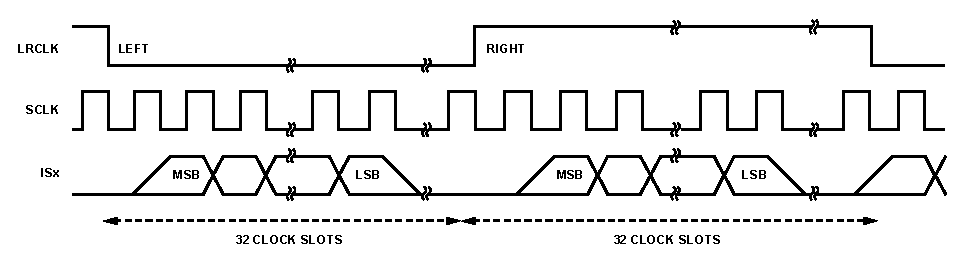
\includegraphics[width=1.0\textwidth]{audio_i2s}
		\caption{Ilustração dos sinais de som transmitidos no formato $I^{2}$S, retirada de \cite{R016}}
		\label{fig:i2s_audio}
	\end{center}
\end{figure}

Na placa recetora HDMI, que envia os dados para a FPGA Virtex-7, é também enviado o sinal \textit{Master Clock} que corresponde a um sinal de relógio de referência do sinais de áudio da entrada e ainda dados de áudio em AP0. É mencionado em \cite{R016} que estes dois sinais são referentes ao som no formato SPDIF e como tal não serão abordados neste projeto uma vez que as placas apenas suportam o formato $I^{2}$S.

Para além de dados de som e imagem são transmitidos dois bits com informação relativa ao estado do vídeo transmitido. Estes dados indicam o tipo e formato de vídeo que está a ser transmitidos e devem de seguida ser recebidos na placa transmissora. A combinação dos dois bits definem o estado do vídeo e são detalhadas em \cite{R014}.

Esta configuração acaba por ser bastante útil e será utilizada em diversas arquiteturas desenvolvidas uma vez que possui duas grandes vantagens: é capaz de suportar som e ao mesmo tempo não limita o formato da imagem transmitida a RGB. Em contrapartida, apenas suporta um canal (ao contrário da anterior), mas tal não é um problema pois apenas se pretende obter a transmissão num único canal entre dispositivo de fonte e dispositivo final HDMI. 


\subsubsection{Suporte de dois canais de imagem melhorado} \label{subsubsec:HDMIconfigMelhorado}


Esta configuração é capaz de suportar a transmissão de imagens em dois canais, tal como a configuração apresentada em \ref{subsubsec:HDMIconfigdefault} no entanto com alguns melhoramentos. A principal diferença consiste na capacidade de transmitir não só imagens em formato RGB mas também em YCbCr num dos canais. A tabela \ref{table:HDMI1canal_melhorado} do anexo \ref{ap1:HDMI} foi adaptada de \cite{R013} e apresenta detalhadamente todos os sinais transmitidos entre as placas HDMI e ainda os nomes dos conectores FMC.

Esta configuração na placa recetora transmite no canal 0 (RX0)  imagens tanto no formato RGB como YCbCr de 10 bits por cor e os sinais de controlo respectivos. Relativamente ao canal 1 dessa mesma placa (RX1) apenas é possível transmitir imagens em formato RGB de 10 bits por cor e os seus respetivos controlos. Para além disso, para cada canal são transmitidos dois bits que identificam o estado do vídeo que é transmitido, tal como já acontecia na configuração descrita em \ref{subsubsec:HDMIconfig+audio}.

Quando à placa transmissora quando configurada desta forma é capaz de receber nos dois canais (TX0 e TX1) imagens no formato RGB ou YCbCr com 10 bits por cor. Apesar de na tabela \ref{table:HDMI1canal_melhorado} o canal 1 definir os seus bits apenas para o caso de RGB, este canal também suporta na placa transmissora o formato YCbCr (e por isso a atribuição dos bits para TX1 assemelham-se ao canal TX0). Tal não é suportado no canal 1 da placa HDMI recetora (RX1) e por esse motivo a tabela está assim apresentada. À semelhança da placa recetora, a placa transmissora recebe 2 bits relativos à informação do vídeo que está a ser transferido, tal como a tabela \ref{table:HDMI1canal_melhorado} sugere.

\subsection{Configuração dos interruptores}

Neste capitulo serão descritas as configurações dos interruptores presentes nas placas HDMI para cada configuração existente. Tal é necessário definir para que os recetores e transmissores presentes nas placas possam enviar e receber imagens nos formatos que o utilizador pretende. Existem 8 interruptores que podem ser definidos pelo utilizador. Os interruptores entre S1-1 e S1-4 têm como função selecionar o tipo de formato que sai do recetor ADV7612 ou ADV7511 embebido na placa. Relativamente aos outros interruptores, raramente são utilizados e quando são a sua função não é relevante para o projeto e por isso não será especificada.

\subsubsection{Configuração por \textit{default}} \label{subsubsec:HDMIconfigdefault_switches}

Quando as placas estão configuras de fábrica, relembra-se que as imagens transmitidas correspondem ao formato RGB de 30 bits (10 bits por cor). Como tal, a indicação que vem em \cite{R009} sobre as funções dos interruptores da placa HDMI recetora é muito pouca. Apenas é indicado que quando esta configuração está ativa os interruptores se devem encontrar tal como especifica a tabela \ref{table:HDMI_default_switches_RX} na página \pageref{table:HDMI_default_switches_RX}.

\begin{table}[h!]
	\centering
	\begin{tabular}{|c|c|}
		\hline
		\textbf{Interruptor} & \textbf{Estado} \\ \hline
		\textbf{S1-1}        & ON              \\ \hline
		\textbf{S1-2}        & ON              \\ \hline
		\textbf{S1-3}        & ON              \\ \hline
		\textbf{S1-4}        & ON              \\ \hline
		\textbf{S1-5}        & Não usado       \\ \hline
		\textbf{S1-6}        & Não usado       \\ \hline
		\textbf{S1-7}        & Não usado       \\ \hline
		\textbf{S1-8}        & ON              \\ \hline
	\end{tabular}
	\caption{Configuração dos interruptores da placa HDMI RX configurada de fábrica, adaptada de \cite{R009}}
	\label{table:HDMI_default_switches_RX}
\end{table}

Relativamente à placa HDMI transmissora, é sabido que lhe chegam imagens no formato RGB de 10 bits, no entanto é possivel configurar o ADV7511 de tal forma que na sua saída o número de bits não seja limitado a 10. Para tal é necessário configurar os interruptores da forma que a tabela \ref{table:HDMI_default_switches_TX} indica.

 \begin{table}[h!]
	\centering
	\begin{tabular}{|c|c|c|c|}
		\hline
		\textbf{Interruptor} & \multicolumn{3}{c|}{\textbf{Estado}} \\ \hline
		\textbf{S1-1}        & OFF        & ON         & ON         \\ \hline
		\textbf{S1-2}        & ON         & ON         & OFF        \\ \hline
		\textbf{S1-3}        & ON         & OFF        & ON        \\ \hline
		\textbf{S1-4}        & ON         & ON         & ON         \\ \hline
		\textbf{OUTPUT}      & 8 bits     & 10 bits    & 12 bits    \\ \hline
		\textbf{S1-5}        & \multicolumn{3}{c|}{OFF}             \\ \hline
		\textbf{S1-6}        & \multicolumn{3}{c|}{Não usado}       \\ \hline
		\textbf{S1-7}        & \multicolumn{3}{c|}{Não usado}       \\ \hline
		\textbf{S1-8}        & \multicolumn{3}{c|}{Não usado}       \\ \hline
	\end{tabular}
	\caption{Configuração dos interruptores da placa HDMI RX configurada de fábrica, adaptada de \cite{R009}}
	\label{table:HDMI_default_switches_TX}
\end{table}
\subsubsection{Suporte de um canal de imagem e áudio} \label {subsubsec:HDMIconfig+audio_switches}

Quando se configuram as placas HDMI de forma a obter-se o suporte de áudio, então o formato da imagem transmitida também não é limitado a RGB. Desta maneira, o tabela \ref{table:HDMI_1ch+audio_switches_RX} indica como se devem configurar os interruptores de forma a obter-se na saída do ADV7612 as diversas possibilidades relativamente ao formato da imagem.
\begin{table}[h!]
	\centering
	\begin{tabular}{|c|c|c|c|c|c|c|}
		\hline
		\textbf{Interruptor}             & \multicolumn{6}{c|}{\textbf{Estado}}                                                                                                                                                                           \\ \hline
		\textbf{S1-1}                    & ON                                                        & OFF                                                       & ON                                                        & ON     & OFF     & ON      \\ \hline
		\textbf{S1-2}                    & ON                                                        & ON                                                        & OFF                                                       & ON     & ON      & OFF     \\ \hline
		\textbf{S1-3}                    & ON                                                        & ON                                                        & ON                                                        & OFF    & OFF     & OFF     \\ \hline
		\textbf{S1-4}                    & ON                                                        & ON                                                        & ON                                                        & ON     & ON      & ON      \\ \hline
		\multirow{2}{*}{\textbf{OUTPUT}} & \begin{tabular}[c]{@{}c@{}}YCbCr\\   444/422\end{tabular} & \begin{tabular}[c]{@{}c@{}}YCbCr\\   444/422\end{tabular} & \begin{tabular}[c]{@{}c@{}}YCbCr\\   444/422\end{tabular} & RGB    & RGB     & RGB     \\ \cline{2-7} 
		& 8 bits                                                    & 10 bits                                                   & 12 bits                                                   & 8 bits & 10 bits & 12 bits \\ \hline
		\textbf{S1-5}                    & \multicolumn{6}{c|}{ON}                                                                                                                                                                                        \\ \hline
		\textbf{S1-6}                    & \multicolumn{6}{c|}{ON}                                                                                                                                                                                        \\ \hline
		\textbf{S1-7}                    & \multicolumn{6}{c|}{ON}                                                                                                                                                                                        \\ \hline
		\textbf{S1-8}                    & \multicolumn{6}{c|}{ON}                                                                                                                                                                                        \\ \hline
	\end{tabular}
	\caption{Configuração dos interruptores da placa HDMI RX configurada para um canal e suporte de áudio, adaptada de \cite{R014}}
	\label{table:HDMI_1ch+audio_switches_RX}
\end{table}

À semelhança da placa recetora para esta configuração, também é possivel configurar o ADV7511 para se obter na sua saída diversos formatos de imagem. A tabela \ref{table:HDMI_1ch+audio_switches_TX} apresentada na página \pageref{table:HDMI_1ch+audio_switches_TX} indica essas mesmas combinações. 
\begin{table}[h!]
	\centering
	\begin{tabular}{|c|c|c|c|c|c|c|c|c|c|}
		\hline
		\textbf{Interruptor}             & \multicolumn{9}{c|}{\textbf{Estado}}                                                                                                                                                                                                                                                                                                                                       \\ \hline
		\textbf{S1-1}                    & ON                                                    & OFF                                                   & ON                                                    & ON                                                    & OFF                                                   & ON                                                    & ON     & OFF     & ON      \\ \hline
		\textbf{S1-2}                    & ON                                                    & ON                                                    & OFF                                                   & ON                                                    & ON                                                    & OFF                                                   & ON     & ON      & OFF     \\ \hline
		\textbf{S1-3}                    & ON                                                    & ON                                                    & ON                                                    & OFF                                                   & OFF                                                   & OFF                                                   & ON     & ON      & ON      \\ \hline
		\textbf{S1-4}                    & ON                                                    & ON                                                    & ON                                                    & ON                                                    & ON                                                    & ON                                                    & OFF    & OFF     & OFF     \\ \hline
		\multirow{2}{*}{\textbf{OUTPUT}} & \begin{tabular}[c]{@{}c@{}}YCbCr\\   444\end{tabular} & \begin{tabular}[c]{@{}c@{}}YCbCr\\   444\end{tabular} & \begin{tabular}[c]{@{}c@{}}YCbCr\\   444\end{tabular} & \begin{tabular}[c]{@{}c@{}}YCbCr\\   422\end{tabular} & \begin{tabular}[c]{@{}c@{}}YCbCr\\   422\end{tabular} & \begin{tabular}[c]{@{}c@{}}YCbCr\\   422\end{tabular} & RGB    & RGB     & RGB     \\ \cline{2-10} 
		& 8 bits                                                & 10 bits                                               & 12 bits                                               & 8 bits                                                & 10 bits                                               & 12 bits                                               & 8 bits & 10 bits & 12 bits \\ \hline
		\textbf{S1-5}                    & \multicolumn{9}{c|}{OFF}                                                                                                                                                                                                                                                                                                                                                   \\ \hline
		\textbf{S1-6}                    & \multicolumn{9}{c|}{Não usado}                                                                                                                                                                                                                                                                                                                                             \\ \hline
		\textbf{S1-7}                    & \multicolumn{9}{c|}{Não usado}                                                                                                                                                                                                                                                                                                                                             \\ \hline
		\textbf{S1-8}                    & \multicolumn{9}{c|}{ON}                                                                                                                                                                                                                                                                                                                                                    \\ \hline
	\end{tabular}
	\caption{Configuração dos interruptores da placa HDMI TX configurada para um canal e suporte de áudio, adaptada de \cite{R014}}
	\label{table:HDMI_1ch+audio_switches_TX}
\end{table}

\subsubsection{Suporte de dois canais de imagem melhorado} \label{subsubsec:HDMIconfigMelhorado_switches}

Quando se reconfigura as placas para suportarem a versão de transmissão de dois canais melhorada, é necessário ter em conta que existe um canal (canal 0) que tem a possibilidade de transmitir imagens tanto no formato YCbCr como RGB, porém o canal 1 apenas o faz no formato RGB. Na tabela \ref{table:HDMI_2ch_melhoradp_RX} da página \pageref{table:HDMI_2ch_melhoradp_RX} são apresentadas as configurações dos interruptores que configuram o ADV7612 de forma a enviar diferentes formatos.

\begin{table}[h!]
	\centering

	\begin{tabular}{|c|c|c|c|c|}
		\hline
		\textbf{Interruptor}             & \multicolumn{4}{c|}{\textbf{Estado}}             \\ \hline
		\textbf{S1-1}                    & ON            & OFF           & ON     & OFF     \\ \hline
		\textbf{S1-2}                    & ON            & ON            & ON     & ON      \\ \hline
		\textbf{S1-3}                    & ON            & ON            & OFF    & OFF     \\ \hline
		\textbf{S1-4}                    & ON            & ON            & ON     & ON      \\ \hline
		\multirow{2}{*}{\textbf{OUTPUT}} & YCbCr 444/422 & YCbCr 444/422 & RGB    & RGB     \\ \cline{2-5} 
		& 8 bits        & 10 bits       & 8 bits & 10 bits \\ \hline
		\textbf{S1-5}                    & \multicolumn{4}{c|}{ON}                          \\ \hline
		\textbf{S1-6}                    & \multicolumn{4}{c|}{ON}                          \\ \hline
		\textbf{S1-7}                    & \multicolumn{4}{c|}{ON}                          \\ \hline
		\textbf{S1-8}                    & \multicolumn{4}{c|}{ON}                          \\ \hline
	\end{tabular}
	\caption{Configuração dos interruptores da placa HDMI RX configurada para dois canais melhorados, adaptada de \cite{R013}}
	\label{table:HDMI_2ch_melhoradp_RX}
\end{table}

Relativamente à placa HDMI transmissora, ambos os canais são capazes de suportar imagens em formato RGB ou YCbCr. A tabela \ref{table:HDMI_2ch_melhoradp_TX} da página \pageref{table:HDMI_2ch_melhoradp_TX} apresenta as combinações dos interruptores para se poder obter os diversos formatos na saída do ADV7511.
\begin{table}[h!]
	\centering
	\begin{tabular}{|c|c|c|c|c|c|c|}
		\hline
		\textbf{Interruptor}             & \multicolumn{6}{c|}{\textbf{Estado}}                             \\ \hline
		\textbf{S1-1}                    & ON        & OFF       & ON        & OFF       & ON     & OFF     \\ \hline
		\textbf{S1-2}                    & ON        & ON        & ON        & ON        & ON     & ON      \\ \hline
		\textbf{S1-3}                    & ON        & ON        & OFF       & OFF       & ON     & ON      \\ \hline
		\textbf{S1-4}                    & ON        & ON        & ON        & ON        & OFF    & OFF     \\ \hline
		\multirow{2}{*}{\textbf{OUTPUT}} & YCbCr 444 & YCbCr 444 & YCbCr 422 & YCbCr 422 & RGB    & RGB     \\ \cline{2-7} 
		& 8 bits    & 10 bits   & 8 bits    & 10 bits   & 8 bits & 10 bits \\ \hline
		\textbf{S1-5}                    & \multicolumn{6}{c|}{OFF}                                         \\ \hline
		\textbf{S1-6}                    & \multicolumn{6}{c|}{Não usado}                                   \\ \hline
		\textbf{S1-7}                    & \multicolumn{6}{c|}{Não usado}                                   \\ \hline
		\textbf{S1-8}                    & \multicolumn{6}{c|}{ON}                                          \\ \hline
	\end{tabular}
	\caption{Configuração dos interruptores da placa HDMI RX configurada para dois canais melhorados, adaptada de \cite{R013}}
	\label{table:HDMI_2ch_melhoradp_TX} 
\end{table}
\section{Arquiteturas Desenvolvidas} \label{sec:HDMIarquiteturas}

Nesta secção passam a ser descritas as arquiteturas desenvolvidas e implementadas na FPGA referentes à comunicação entre as placas HDMI.  Por outras palavras, é feita uma aplicação daquilo que foi explicado sobre as placas HDMI a serem utilizadas até agora em arquiteturas implementadas e testadas em FPGA.

\subsection{Transmissão de uma imagem gerada na FPGA} \label{subsub:planA}

Numa fase inicil do projeto, optou-se por simplificar a transmissão e para tal utilizou-se apenas a placa transmissora HDMI configurada por defeito. Contrui-se em Verilog um bloco capaz de gerar uma imagem para ser transmitida, mais especificamente uma barra de cores, e utlizou-se essa imagem para ser transmitida pelos conectores FMC.

O bloco gerador de uma barra de cores foi adaptado de um bloco disponibilizado pela \textit{Inrenvium} aquando a compra das placas. Apesar de ter sido ligeiramente adaptado para este caso em especifico, este baseia-se essencialmente numa maquina de estados que vai contando as linhas e as colunas para que possa enviar não só os valores das cores de cada pixel, mas também os sinais de controlo como a sincronização vertical, a sincronização horizontal e ainda os valor de pixeis ativos.

Para que se entenda mais facilmente como e quando se transmitem os sinais de controlo da imagem e também os valor dos pixeis é demonstrado na imagem \ref{fig:colorBar_exemple} na página \pageref{fig:colorBar_exemple} uma exemplo de transmissão de uma imagem gerada na FPGA. Antes de passar para descrição da geração da imagem passam a ser descritos os acrónimos apresentados na figura:

\begin{enumerate}
	\item \textbf{HRES:} \textit{Horizontal Resolution} é o parâmetro que define a resolução horizontal da imagem que vai ser gerada pelo bloco, ou seja o número de pixeis em cada linha de transmissão.
	\item \textbf{HSW:} \textit{Horizontal Sync Width} é o parâmetro que define o número de ciclos de relógio que o sinal de sincronização horizontal tem.
	\item \textbf{HBP:} \textit{Horizontal Back Porch} é o parâmetro que define o número de pixeis que não contêm informação útil (relativamente à cor dos mesmos) antes de começar a ser transmitida a linha de imagem.
	\item \textbf{HFP:} \textit{Horizontal Front Porch} é o parâmetro que define o número de pixeis que não contem informação útil depois de ser transmitida uma linha da imagem.
	\item \textbf{VRES:} \textit{Vertical Resolution} é o parâmetro que define a resolução vertical da imagem que vai ser gerada pelo bloco, por outras palavras é o número de linhas de pixeis a ser geradas.
	\item \textbf{VSW:} \textit{Vertical Sync Width} é o parâmetro que define o número de linhas horizontais que o sinal de sincronização vertical está ativo.
	\item \textbf{VBP:} \textit{Vertical Back Porch} é o parâmetro que define o número de linhas horizontais que não contém informação útil relativamente ao pixeis antes de começarem a ser transmitidas as linhas de pixeis.
	\item \textbf{VFP:} \textit{Vertical Front Porch} é o parâmetro que define o número de linhas horizontais que não contém informação útil relativamente ao pixeis depois de terem sido transmitidas todas as linhas horizontais da imagem.
\end{enumerate}
	
\begin{figure}[h!]
	\begin{center}
		\leavevmode
		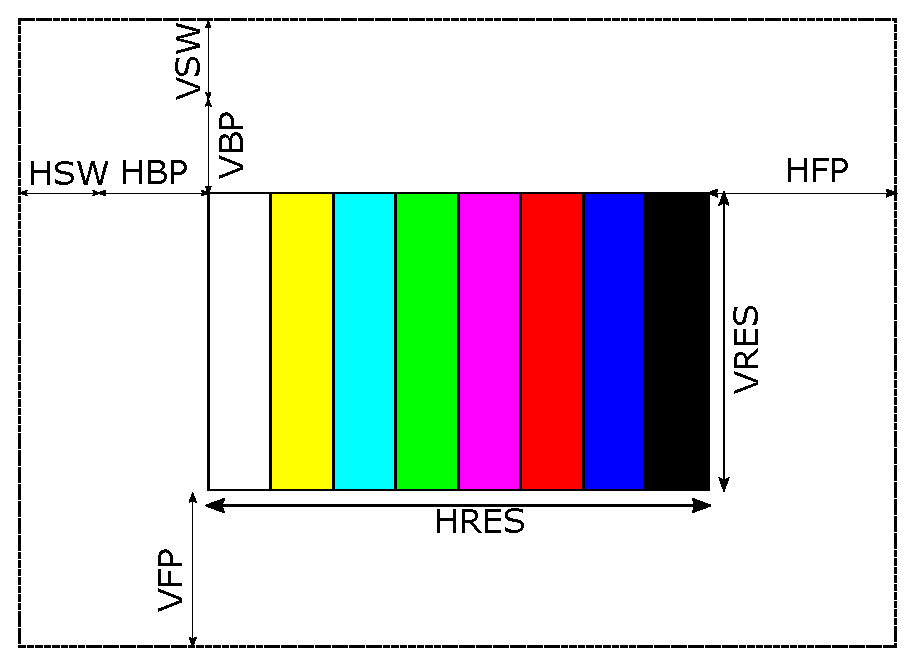
\includegraphics[width=1.0\textwidth]{exemplo_colorBar}
		\caption{Exemplo de imagem gerada pelo modulo desenvolvido}
		\label{fig:colorBar_exemple}
	\end{center}
\end{figure}

Para gerar uma imagem em \textit{FULL HD} cuja resolução é 1920x1080 pixeis e o sinal de relógio deve ter uma frequência de 148.5 MHz, foram o utilizados os seguintes valores para os parâmetro previamente descritos: HRES = 1920, HSW = 44, HBP = 44, HFP = 148,  VRES = 1080, VSW = 5, VBP = 36 e VFP = 4.

A figura \ref{fig:colorBar_fsm} na página \pageref{fig:colorBar_fsm} ilustra a maquina de estados desenvolvida para implementar a geração de uma barra a cores na FPGA. 

\begin{figure}[h!]
	\begin{center}
		\leavevmode
		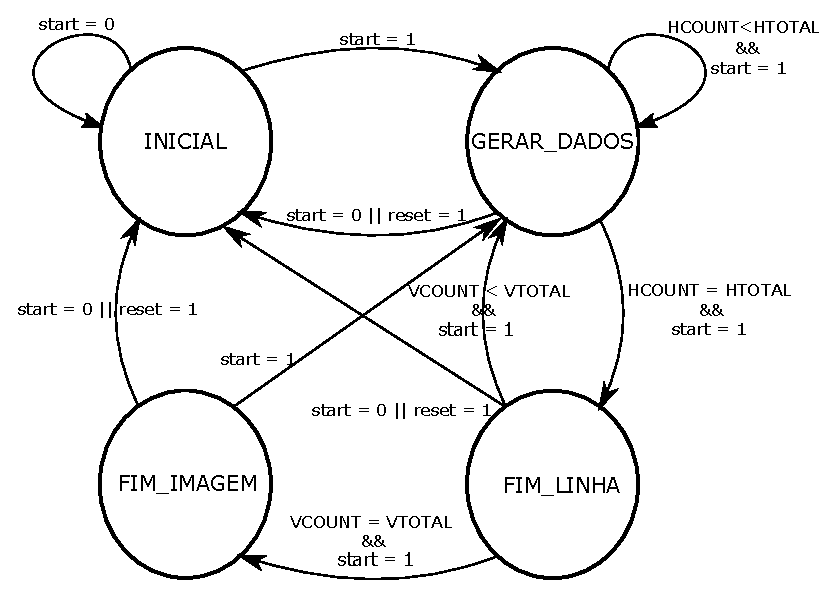
\includegraphics[width=1.0\textwidth]{colorBar_FSM}
		\caption{Máquina de estados para gerar uma barra de cores}
		\label{fig:colorBar_fsm}
	\end{center}
\end{figure}

Os registos VCOUNT E HCOUNT de decisão que se visualiza na figura correspondem a contadores que vão contanto pixel a pixel até ao fim de uma linha (no caso do HCOUNT) ou então de uma imagem inteira (no caso do VCOUNT). Os valores de HTOTAL e VTOTAL não são mais do que a soma de todo o tamanho dos dados na horizontal e na vertical respectivamente. Assim sendo, para este caso em especifico obtem-se os seguintes valores:
\begin{itemize}
	\item HTOTAL = HSW + HBP + HRES + HFP = 44 + 44 + 1920 + 148 = 2156
	\item VTOTAL = VSW + VBP + VRES + VFP = 5 + 36 + 1080 + 4 = 1125
\end{itemize}

Para além destes sinais de decisão para mudança de estado existem mais dois sinais no diagrama da máquina de estados presente na figura \ref{fig:colorBar_fsm} que ainda não foram mencionados que são o \textit{reset} e o \textit{start}. Estes dois sinais são botões do utilizador que lhe permitem definir quando se pretende que a transmissão esteja ativa ou desativa (através do botão \textit{start}) ou então quando se pretende restabelecer os dados originais da máquina de estados (através do botão \textit{reset}). 


Existem 4 estados nesta máquina eu consistem essencialmente em detecção do final de uma linha, e detecção do final de uma imagem e geração de dados. Os estados passam a ser descritos de seguida:

\begin{enumerate}
	\item \textbf{Estado inicial:} Neste estado são configurados os parâmetros para o inicio de uma transmissão, ou seja, os valores de HCOUNT e VCOUNT são igualados ao valor total do tamanho na horizontal e na vertical respectivamente. Por outras palavras, os valores de HCOUNT e VCOUNT são igualados a HTOTAL e VTOTAL respectivamente. Isto acontece porque é possivel retornar a este estado estando em qualquer um dos outros desde que seja pressionado o botão  de \textit{reset} ou então que a transmissão seja desligada pelo utilizador (\textit{start} = 0).
	\item \textbf{Estado para gerar dados:} Neste estado, ao flanco positivo do sinal de relógio do sistema, é incrementado o valor de HCOUNT e ao mesmo tempo são gerados os dados a serem transmitidos em cada ciclo de sinal de relógio, consoante o valor de HCOUNT e VCOUT. Quando o valor de HCOUNT se igualar ao valor de HTOTAL, então significa que foi transmitida uma linha inteira da imagem, e por isso a máquina transita de estado e o valor de VCOUNT volta a ser igualado a 1. O processo de geração de dados será explicado em XXXX
	\item \textbf{Estado de fim de linha:} Quando este estado está ativo, então uma linha da imagem foi transmitida, o que implica que é necessário incrementar o valor de linhas totais transmitidas (incrementando 1 valor em VCOUNT) e ainda verificar se a transmissão de uma imagem completa está realizada. Caso o valor de VCOUNT se iguale ao valor de VTOTAL, então transita-se para o estado de fim de imagem, e coloca-se o valor de VCOUNT a 1. Caso contrário, então a máquina transita para o estado que estava anteriormente.
	\item \textbf{Estado de fim de imagem} Quando este estado está ativo então significa que ambos os valores de HCOUNT e VCOUNT estão igualados a 1 e que por isso já foi transmitida uma imagem completa e como tal passa-se a transmitir uma próxima imagem, transitando novamente para o estado para gerar dados.
\end{enumerate}

Quando a máquina de estados se encontra no estado para gerar dados, então os dados de controlo são gerados nas seguintes condições :
\begin{itemize}
	\item \textbf{Sinal de sincronização vertical:} O sinal de sincronização vertical é um sinal que como já foi referido anteriormente indica o incio de transmissão de uma nova imagem, e por isso é ativado pela máquina de estados desenvolvida quando o valor em VCOUNT se igual ao valor de VTOTAL e quando o valor de HCOUNT se igual ao valor de HTOTAL, ou seja é ativado no final de uma imagem. Este sinal é ainda desligado quando o valor de VCOUNT se igual a VSW e o valor de HCOUNT se igual ao valor de HTOTAl, isto porque quando estas duas condições se verificam seignifica que o número de linhas em que o sinal de sincronização vertical deve estar ativo já terminou (é mesmo isso que o valor do parâmetro VSW define : \textit{Vertical Sync Width}).
	
	\item \textbf{Sinal de sincronização horizontal:} O sinal de sincronização horizontal indica o inicio de uma nova linha e como tal deve ser ativo sempre que o valor de HCOUNT se igual e ao valor de HTOTAL (porque indica o fim da emissão de uma linha). Da mesma maneira, este sinal deve ser desativo sempre que o valor de HCOUNT se igual ao valor de HSW, isto porque este valor indica que o período de tempo que este sinal deve estar ativo terminou.
	
	\item \textbf{Sinal de dados ativos:} Este sinal deve estar ativo sempre que se estiver a transmitir pixeis válidos, e por isso sempre que as condições que serão de seguida apresentadas se verificarem:
	\begin{enumerate}
		\item O valor de VCCOUNT é maior do que a soma entre VSW e VBP.
		\item O valor de VCOUNT é menor do que a soma entre VSW, VBP, VRES e 1.
		\item O valor de HCOUNT é maior do que a soma entre HSW, HBP subtraída de 1 valor.
		\item O valor de HCOUNT é menor do que a soma HSW, HBP e HRES.
	\end{enumerate}
	As duas primeira condições garantem que VCOUNT está na zona vertical que corresponde à transmissão de imagem na figura \ref{fig:colorBar_exemple}, e as duas ultimas condições garantem o mesmo mas na zona horizontal.
	\item \textbf{Valor dos pixeis:} Estes sinais correspondem a um barramento de 30 bits de uma imagem RGB com 10 bits por componente de cor. Como tal, estes valores devem corresponder a cores sempre o sinal de dados ativos estiver ligado e 0 sempre que estiver desligado. 
\end{itemize}

\begin{figure}[h!]
	\begin{center}
		\leavevmode
		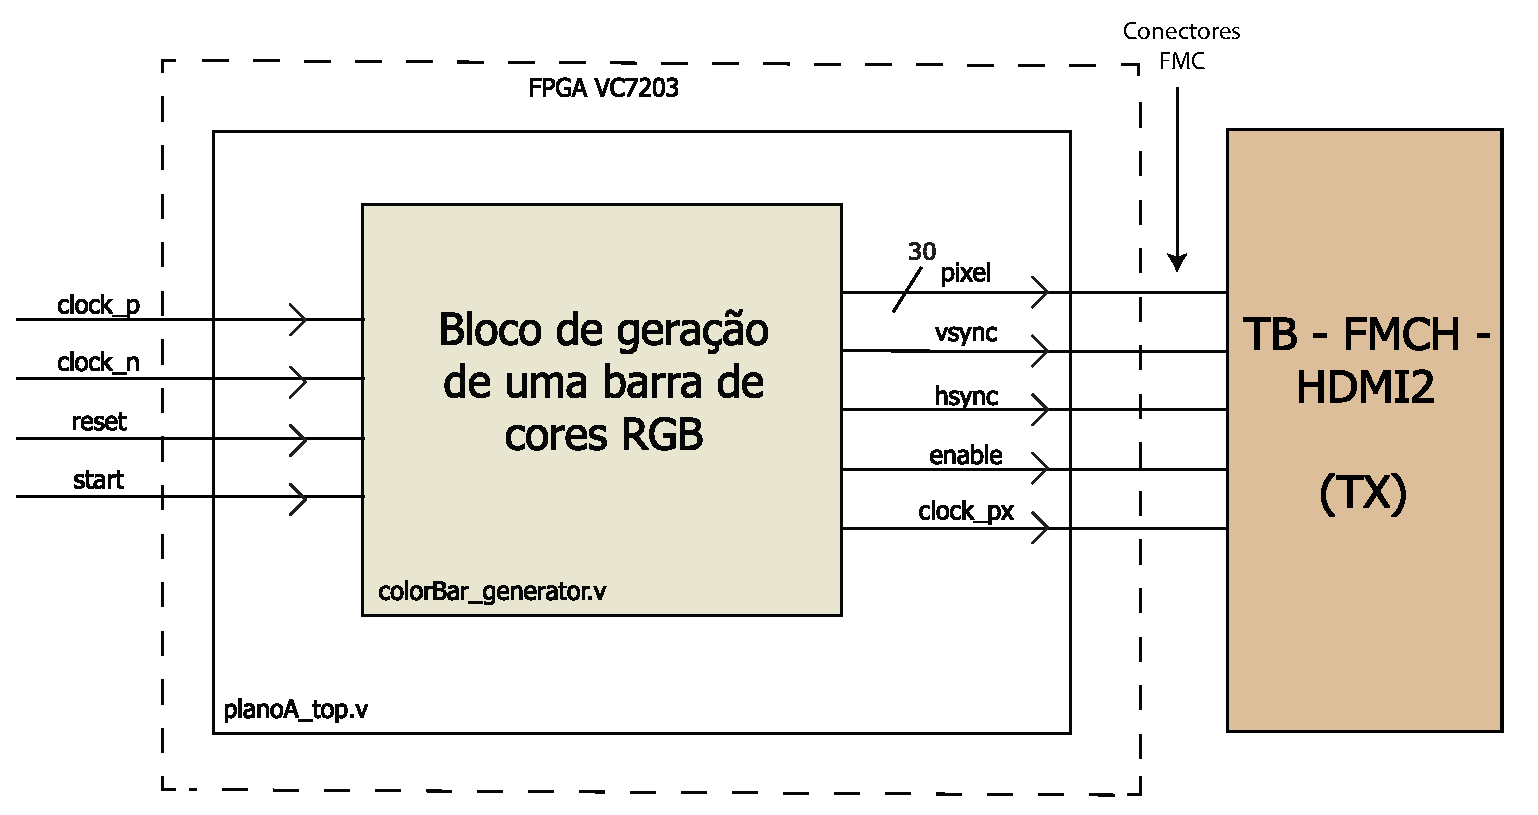
\includegraphics[width=1.0\textwidth]{planA}
		\caption{Diagrama de blocos de arquitetura implementada utilizando um bloco gerador de barra de cores}
		\label{fig:planA}
	\end{center}
\end{figure}

Na figura \ref{fig:planA} é apresentado um diagrama de blocos da arquitetura implementada recorrendo a um bloco gerador de uma barra de cores. Este bloco foi implementado recorrendo-se à maquina de estados apresentada anteriormente.

Nas entradas do bloco estão ligados 4 sinais sendo que dois deles correspondem a um sinal de relógio diferencial de 200 MHz (\textit{clock\_p} corresponde ao sinal positivo e \textit{clock\_n} ao sinal negativo), e os outros dois sinais, \textit{start} e \textit{reset}, são sinais relevantes para a máquina de estados do bloco de geração de barras de cores definidos pelo utilizador e, por isso, são atribuídos a botões da FPGA. O sinal de relógio diferencial ligado às entradas deste bloco é proveniente do oscilador presente na FPGA e irá alimentar uma modulo que coloca na sua saída um sinal de relógio de 148.5 MHz. Esse módulo foi criado através do IP disponibilizado no VIVADO \textit{Clocking Wizard} que vem facilitar a geração de um sinal de relógio com a frequência pretendida tendo como uma base um sinal diferencial de 200 MHz. O sinal gerado, de 148.5 MHz, é o sinal de relógio principal do sistema uma vez que é a frequência necessária para gerar uma imagem em \textit{FULL HD}, e como tal é a essa cadência que os sinais serão enviados para a placa HDMI transmissora e é esse ainda o sinal de relógio da mesma.

Relativamente às saída do módulo é possivel visualizar na imagem \ref{fig:planA} que estas se encontram diretamente ligadas à placa transmissora HDMI através dos conectores FMC. Estes sinais são um barramento de 30 bits que corresponde ao pixel (\textit{pixel}), o sinal de sincronização horizontal (\textit{hsync}), o sinal de sincronização de vertical (\textit{vsync}) e ainda o sinal de dados ativos (\textit{enable}).

Para além do desenvolvimento do código em Verilog é necessário que as portas do modulo de topo, no caso desta arquitetura do modulo "planoA\_top.v", estejam atribuidas a portas físicas da FPGA. Para tal é necessário definir onde estão as localizações das portas na FPGA (LOC) e criar um ficheiro de defina essas mesmas restrições fisicas. A tabela \ref{table:LOCplanA_simples} na página \pageref{table:LOCplanA_simples} indica quais as localizações fisicas de cada porta existente no modulo de topo. No caso das portas que se conectam com a placa HDMI transmissora, estão representadas de forma abreviada, no entanto na tabela \ref{table:locPlanAdetail} do anexo \ref{ap3:LOCs} é possivel encontrar todas as portas com mais detalhes e ainda com informação sobre a ligação à placa HDMI transmissora.

\begin{longtable}[h!]
	{|c|c|c|c|}
	\hline
	\centering
%	\begin{tabular}
		\textbf{I/O} & \textbf{Sinal}        & \textbf{LOC na FPGA} & \textbf{Banco na FPGA} \\ \hline  \endhead
		I            & clk\_p                & E19                  & 38                     \\ \hline
		I            & clk\_n                & E18                  & 38                     \\ \hline
		I            & reset                 & N41                  & 19                     \\ \hline
		I            & start                 & E42                  & 19                     \\ \hline
		O            & cll\_px               & E34                  & 35                     \\ \hline
		O            & enable                & K35                  & 34                     \\ \hline
		O            & vsync                 & L31                  & 34                     \\ \hline
		O            & hsync                 & M32                  & 34                     \\ \hline
		O            & pixel{[}0{]}a{[}29{]} & (Ver anexo)          & 34 e 35                \\ \hline
%	\end{tabular}
	\caption{Localização das portas de entrada e saída da arquitetura}
	\label{table:LOCplanA_simples}
\end{longtable}

O ficheiro com estas restrições fisicas gerado após a atribuição das mesmas é apresentado no sub-capitulo \ref{ap2:planA_physical_cnstrs} do anexo \ref{ap2:codigo}. Para cada porta são atribuídas duas restrições: uma que indica a localização fisica na FPGA da porta e outra que indica a norma da mesma (\textit{IOSTANDARD}). A primeira permite atribuir a um determinado lugar físico da FPGA a porta que se pretende e a segunda define a norma dessa mesma porta para que todas as considerações que se tenham de ser tomadas relativamente a essa porta tenham em conta essa mesma norma.

Para além destas restrições fisicas geradas, são também geradas duas restrições temporais quanto aos sinais de relógio à entrada apresentadas no sub-capitulo \ref{ap2:planA_timing_cnstrs} do anexo \ref{ap2:codigo}. As retrições temporais existentes definem que nas portas de entrada do sinal de relógio diferencial existe um sinal com uma frequência de 200 MHz (periodo de 5ns). Isto porque este sinal de relógio é um sinal primário e como tal é importante que a ferramenta de implementação saiba o seu valor para poder garantir que toda a arquitetura cumpre os requisitos temporais.

Após a definição de todas as restrições e escrita do cófigo em verilg, a arquitetura desenvolvida foi devidamente implementada na FPGA e testada obtendo-se o previsto.

\subsection{Transmissão de imagem entre dispositivos HDMI} \label{subsub:planB}

Na arquitetura desenvolvida que é apresentada neste sub-capitulo são utilizadas as placas HDMI recetora e transmissora ambas configuradas por defeito e procede-se à transmissão de uma imagem entre dispositivos HDMI. O objetivo do desenvolvimento desta arquitetura consiste em obter uma ligação entre dois dispositivos ligados às placas HDMI de uma imagem RGB de 10 bits.

Foi desenvolvida uma arquitetura que recebe à cadência do sinal de relógio HDMI proveniente da placa (neste caso em especifico como é uma imagem \textit{FULL HD} é uma frequência de 148,5 MHz) os o resto dos sinais provenientes da mesma, mais especificamente o valor de \textit{pixel}, \textit{vsync}, \textit{hsync} e \textit{enable}. A imagem \ref{fig:planb1} da página \pageref{fig:planb1} ilustra o diagrama de blocos da arquitetura desenvolvida.

\begin{figure}[h!]
	\begin{center}
		\leavevmode
		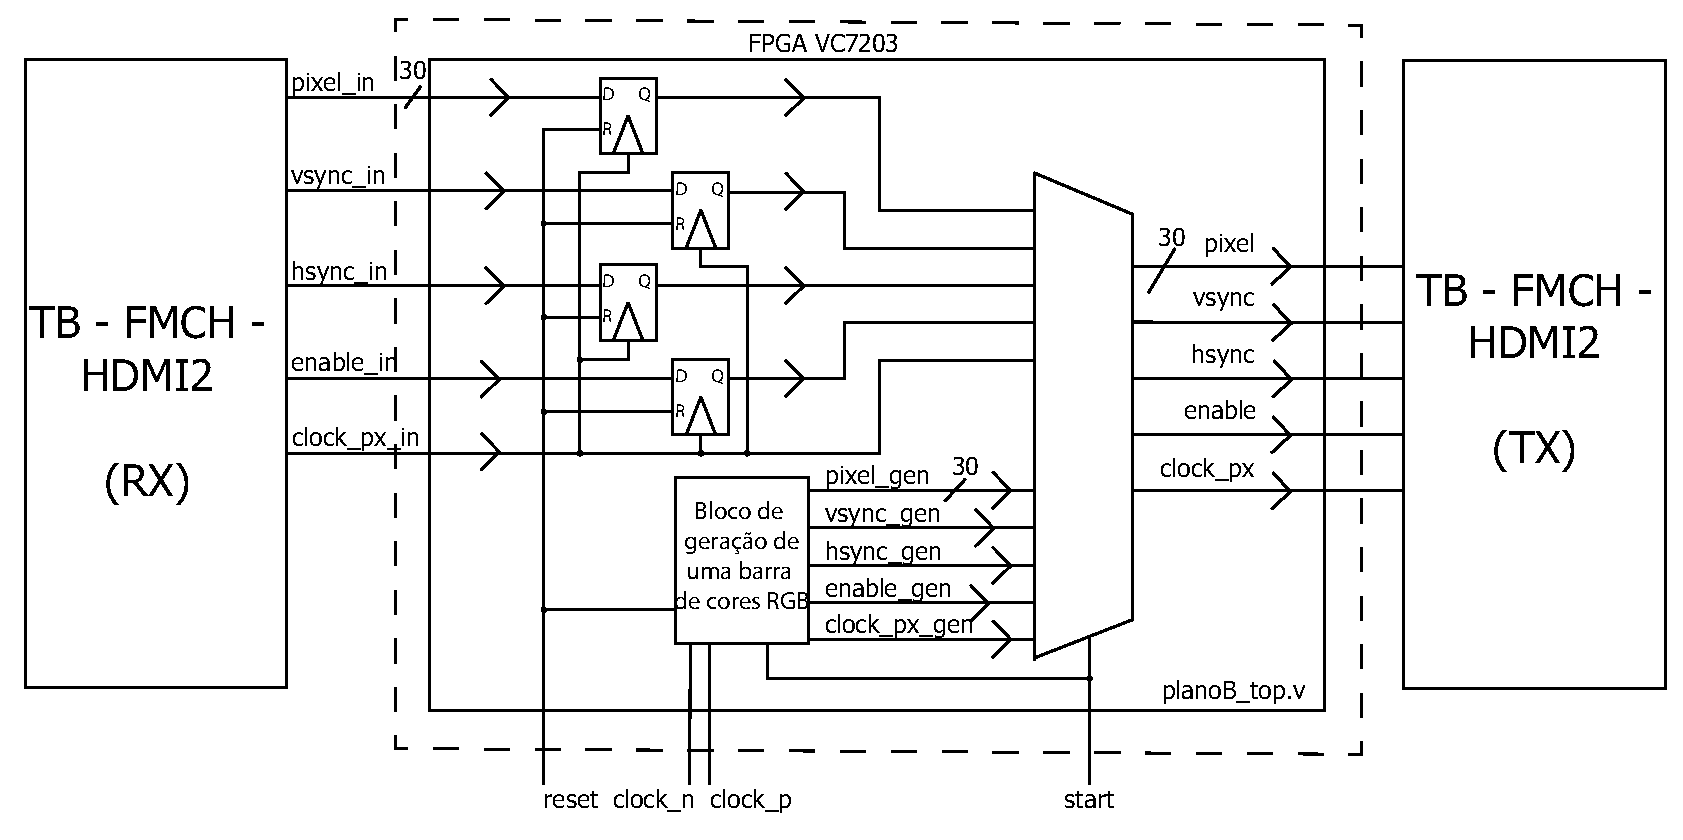
\includegraphics[width=1.0\textwidth]{planB1}
		\caption{Diagram de blocos da arquitetura desenvolvida para transmitir imagem entre dispositivos HDMI}
		\label{fig:planb1}
	\end{center}
\end{figure}
%--> ENTRADA E SAIDA

É possivel visualizar que nesta arquitetura, tal como já acontecia na anterior, existem na sua saída os os sinais que são enviados para a placa HDMI transmisora e para além disso existem também os sinais provenientes da placa HDMI recetora. Também à semelhança da arquitetura descrita em \ref{subsub:planA} existem mais 4 sinais provenientes do exterior: o sinal de relógio diferencia de 200 MHz constituido pelo par positivo \textit{clock\_p} e pelo par negativo \textit{clock\_n}, e ainda o sinal \textit{start} que define o incio da transmissão da barra de cores em vez dos sinais provebientes da fonte HDMI e, por fim, o sinal de \textit{reset} que permite restabelecer os dados originais do sistema caso se pretenda.

%--> FUNCIONAMENTO DA MESMA
Os sinais que são recebidos à entrada são lidos para registos sincronos com o sinal de relógio proveniente da entrada (da placa HDMI recetora). Quando o sinal definido pelo utilizador \textit{start} está ativo os sinais seleccionados pelo multiplexador visivel na figura \ref{fig:planb1} são os sinais provenientes do modulo desenvolvido anteriormente que gera uma barra de cores. Esse mesmo sinal de start está ligado à entrada do bloco gerador da barra de cores para que quando ativo gere a imagem. Quando o sinal \textit{start} está desativo então obtém-se uma ligação entre as placas HDMI recetora e transmissora pois os sinais seleccionados pelo multiplexador são o sinais provenientes da entrada do modulo. Sempre que o sinal de \textit{reset} é ativo então todos os dados são repostos aos originais, como por exemplo os registos voltam ao estado original e também o bloco que produz a barra de cores.

A tabela \ref{table:LOCplanB_simples} na página \pageref{table:LOCplanB_simples} especifica as localizações fisicas da FPGA que foram atribuidas a cada porta do modulo desenvolvido e ainda o banco ao qual pertencem. As portas que fazem conexão com as placas HDMI transmissora e recetora são apresentadas nesta tabela de forma abreviada, no entanto na tabela \ref{table:LOCplanB_detail} do anexo \ref{ap3:LOCs} é possivel encontrar mais detalhamente as localizações dessas portas na FPGA bem como informação relativamente a esses sinais nas placas HDMI transmissora e recetora.

\begin{longtable}[h!]
	{|c|c|c|c|}
	\hline
	\centering
		\textbf{I/O} & \textbf{Sinal}              & \textbf{LOC na FPGA} & \textbf{Banco na FPGA} \\ \hline \endhead
		I            & clk\_p                      & E19                  & 38                     \\ \hline
		I            & clk\_n                      & E18                  & 38                     \\ \hline
		I            & reset                       & N41                  & 19                     \\ \hline
		I            & start                       & E42                  & 19                     \\ \hline
		I            & clk\_px\_in                 & AJ32                 & 14                     \\ \hline
		I            & enable\_in                  & AN38                 & 15                     \\ \hline
		I            & vsync\_in                   & AU38                 & 15                     \\ \hline
		I            & hsync\_in                   & AU39                 & 15                     \\ \hline
		I            & pixel\_in{[}0{]} a {[}29{]} & (Ver anexo)          & 14 e 15                \\ \hline
		O            & clock\_px                   & E34                  & 35                     \\ \hline
		O            & enable                      & K35                  & 34                     \\ \hline
		O            & vsync                       & L31                  & 34                     \\ \hline
		O            & hsync                       & M32                  & 34                     \\ \hline
		O            & pixel{[}0{]}a{[}29{]}       & (Ver anexo)            & 34 e 35                \\ \hline
		\caption{Localização das entradas e saídas das portas da arquitetura}
	\label{table:LOCplanB_simples}
\end{longtable}

%--> CONSTRAINTS %

A atribuição destas mesmas localizações das portas gerou um ficheiro de restrições físicas que é apresentado na secção \ref{ap2:planB_physical_cnstrs} do anexo \ref{ap2:codigo}. Relativamente a estas retrições físicas, existem para cada porta do modulo duas restrições: uma que define a localização fisica e outra a norma da fisica, tal como já foi mencionado anteriormente. 

Quanto às restrições temporais aplicadas ao sistema são idênticas às mesmas aplicadas na arquitetura desenvolvida anteriormente e estáo presentes em \ref{ap2:planB_timing_cnstrs} no anexo \ref{ap2:codigo}.
%--> RESULTADOS

Após sintese e implementação do código desenvolvido em verilog juntamente com as restrições aplicadas, a FPGA foi programada com esta arquitetura e foram obtidos os resultados esperados: obteve-se uma transmissão de imagem entre dois dispositivos HDMI. Foi utilizado um computador com saída HDMI como fonte de imagem conectado a placa HDMI RX, e desta maneira obteve-se no dispositivo HDMI de destino, que neste caso foi um monitor com entrada HDMI, conectado à placa HDMI transmissora a imagem transmitida.


\subsection{Transmissão de imagem e som entre dispositivos HDMI}

Após se obter uma ligação entre dois dispositivos HDMI de uma imagem, procedeu-se ao desenvolvimento de uma arquitetura capaz de trasmitir imagem e som. Para tal foi necessário reconfigurar as placas HDMI, tal como mencionado anteriormente, para a configuração que suporta apenas um canal mas que permite a transmissão de áudio em formato $I^{2}$S. As características desta configuração são apresentadas na secção \ref{subsubsec:HDMIconfig+audio} na página \pageref{subsubsec:HDMIconfig+audio} deste documento, mas é de notar que as imagens poderão ser transmitidas e recebidas em dois tipos de formatos (RGB ou YCbCr) e ainda com 8, 10 ou 12 bits por cor (dependendo da configuração dos interruptores das placas HDMI que estão especificados no sub-capitulo \ref{subsubsec:HDMIconfig+audio_switches}). Neste caso em especifico serão utilizados 12 bits por cor o que preferá um total de 36 bits por pixel.

Na imagem \ref{fig:planC} na página \pageref{fig:planC} é ilustrado um diagrama de blocos da arquitetura desenvolvida para se realizar a transmissão de imagem e som entre dois dispositivos HDMI. 

\begin{figure}[h!]
	\begin{center}
		\leavevmode
		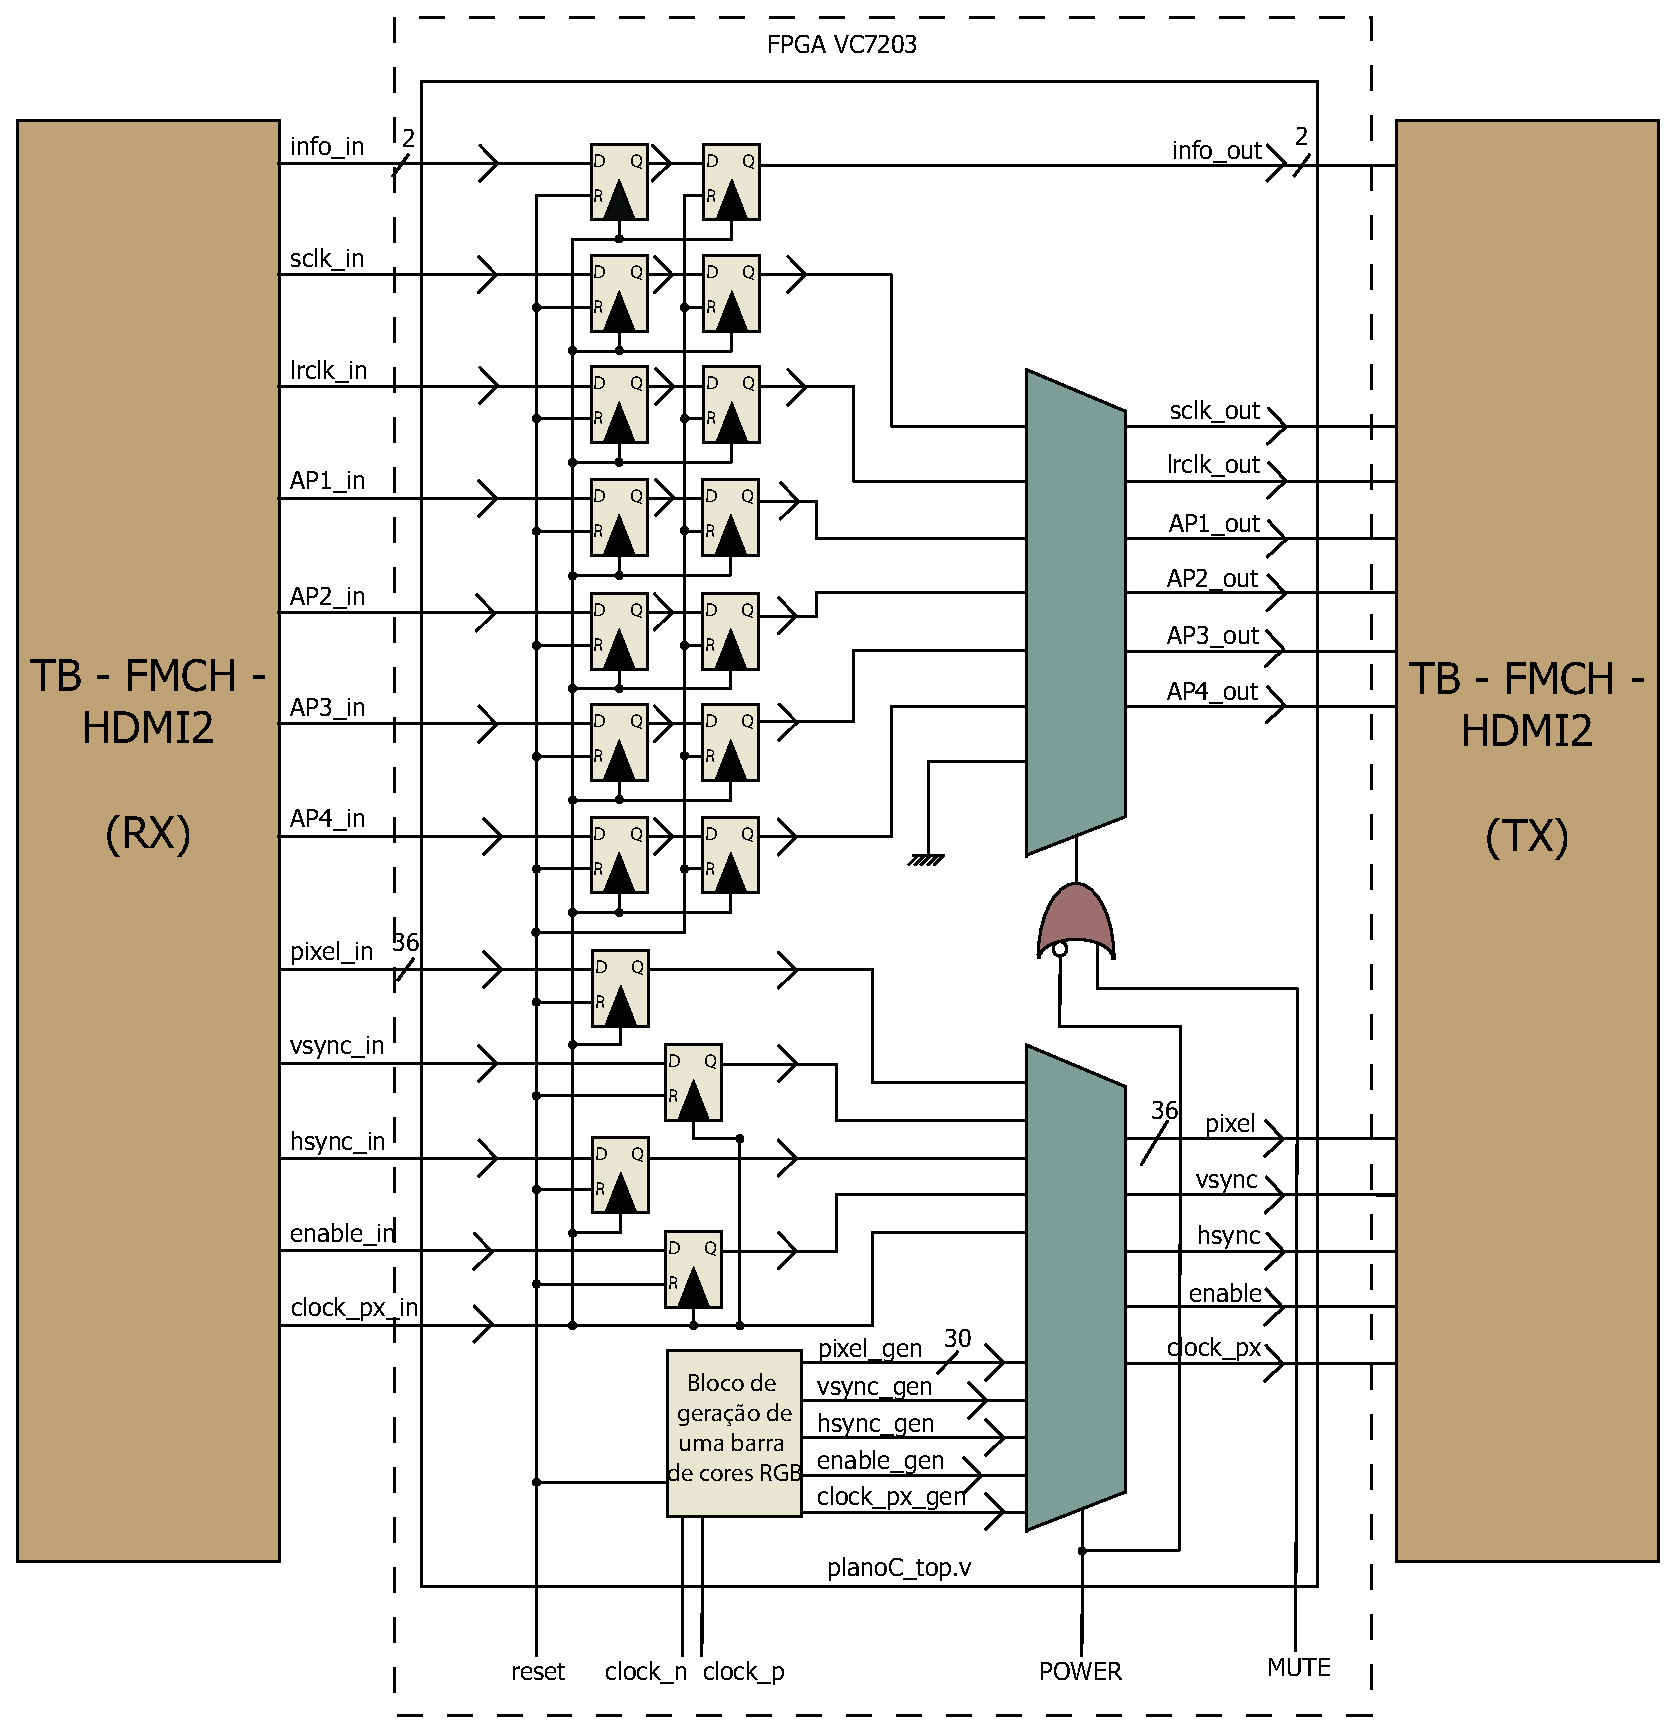
\includegraphics[width=1.0\textwidth]{planC}
		\caption{Diagrama de blocos da arquitetura desenvolvida para transmitir imagem e som entre dispositivos HDMI}
		\label{fig:planC}
	\end{center}
\end{figure}

%--> ENTRADA E SAIDA
Através de uma breve observação do diagrama de blocos ilustrado é possivel concluir que existem mais portas tanto de entrada como de saída nesta arquitetura comparativamente às arquiteturas descritas previamente. Isto deve-se ao facto de agora haver a transmissão do som o que implica a transmissão de mais sinais. Assim sendo, na entrada encontram-se os sinais relativos às imagens à semelhança das arquiteturas anteriores: 36 bits de pixel, sinais de sincronização horizontal\textit{hsync} e vertical (\textit{vsync}) e ainda sinal que indica sinais de pixel ativos(\textit{enable}). Para além destes sinais provenientes da placa HDMI recetora, são recebidos os sinais referentes ao som: o sinal de relógio dos dados em série (\textit{sclk}), o sinal referente à seleccção do canal de audio esquerdo ou direto (\textit{lrclk}) e ainda os sinais que transportam os dados de som (de AP1 a AP4). Para além de dados de imagem e som há também um barramento de 2 bits que contém informação relativamente ao tipo de video que é transmitido (tal como já referido na secção \ref{subsubsec:HDMIconfig+audio}). Todos estes sinais que se encontram na entrada do modulo encontram-se também na saída pois é necessário enviar todos para a placa HDMI transmissora, no entanto o processo de transmissão dos mesmos passa a ser descrito.

Para além destes sinais provenientes e que são enviados para as palcas HDMI existem ainda mais portas do bloco. Existe o tipico sinal de relógio diferencia de 200 MHz definido na porta com \textit{clock\_p} pelo sinal positivo e como \textit{clock\_n} pelo sinal negativo. Este sinal de relógio proveniente do oscilador da FPGA serve como fonte para poder ser reproduzido o sinal de 148.5 MHz (frequência de uma imagem \textit{FULL HD}) que irá produzir a barra de cores no modulo "\textit{coloBar\_generator}". As outras três portas ainda não mencionadas são três sinais definidos pelo utilizador através de interruptores e botões. O sinal de \textit{reset} serve para repor todos os dados originais do sistema caso o utilizador pretenda. O sinal \textit{POWER} é o sinal que define a transmissão dos dados provenientes da placa HDMI recetora ou então da barra de cores, e o sinal \textit{MUTE} define a transmissão ou não dos sinais de som.

%% FUNCIONAMENTO DA MESMA

Os sinais de entrada relativos à imagem, tal como nas arquiteturas anteriores, são lidos para registos síncronos com o sinal de relógio de imagem (que no caso desta demonstração será 148.5 MHz pois são transmitidas imagens em \textit{FULL HD}). Estes mesmo sinais são enviados para a placa HDMI transmissora caso o sinal \textit{POWER} esteja ativo. Este sinal é um sinal que quando está desativo em vez de enviar para as saídas do modulo os sinais recebidos da placa HDMI recetora, envia os dados provenientes do bloco que reproduz uma barra de cores.

Relativamente aos dados referentes ao som, estes são também lidos para registos síncronos com o sinal de relógio referente à imagem proveniente da fonte HDMI pois numa fase mais avançada do projeto tal simplificação virá facilitar a transmissão dos dados em série a alta velocidade. Porém é necessário ter em consideração que estes dados variam a uma taxa que não é síncrona com o sinal de relógio da imagem, pois este possui uma frequência de 148,5 MHz para uma imagem no formato \textit{FULL HD}, e os dados de som variam a uma frequência de 3,072 MHz (tal como mencionado no sub-capitulo \ref{subsubsec:HDMIconfig+audio}). Assim sendo é necessário tomar as devidas precauções quando se faz o cruzamento entre estes dois domínios de relógio para que não sejam captados dados dos registos quando estes se encontram num estado de meta-estabilidade. Assim sendo, tal como sugerido em \cite{R024}, são utilizados dois registos síncronos com o sinal de relógio referente à imagem para que não haja propagações de erros.

O sinal de áudio enviado para as placas HDMI transmissora está dependente do valor do sinal de \textit{POWER} e \textit{MUTE}. Caso \textit{MUTE} esteja ativo o sinal de som não é transmitido e as entradas da placa HDMI são definidas com zero. O mesmo acontece quando o sinal de \textit{POWER} esteja desativo uma vez que indica que a transmissão da parte da placa HDMI recetora está desligada.

Mais uma vez é necessário definir as localizações fisicas de cada porta de entrada e saída do modulo principal, e como tal é possivel encontrar descritas essas mesmas atribuições na tabela \ref{table:LOCplanC_simples} na página \pageref{table:LOCplanC_simples}. Nessa mesma tabela os sinais que se conectam as placas HDMI são brevemente descritas, no entanto na tabela \ref{table:LOCplanC_detail} do anexo \ref{ap3:LOCs} essas mesmas conexões são descritas com mais detalhe.

\begin{longtable}[h!]
	{|c|c|c|c|}

		\hline
		\centering
\textbf{I/O} & \textbf{Sinal}               & \textbf{LOC na FPGA} & \textbf{Banco na FPGA} \\ \hline \endhead
I            & clk\_p                       & E19                  & 38                     \\ \hline
I            & clk\_n                       & E18                  & 38                     \\ \hline
I            & reset                        & N41                  & 19                     \\ \hline
I            & POWER                        & E42                  & 19                     \\ \hline
I            & MUTE                         & G41                  & 19                     \\ \hline
I            & clock\_p\_in                 & AJ32                 & 14                     \\ \hline
I            & vsync\_in                    & AU38                 & 15                     \\ \hline
I            & hsync\_in                    & AU39                 & 15                     \\ \hline
I            & enable\_in                   & AN38                 & 15                     \\ \hline
I            & pixel\_in{[}0{]} a {[}35{]}  & (Ver anexo)          & 14 e 15                \\ \hline
I            & sclk\_in                     & AJ37                 & 14                     \\ \hline
I            & lrclk\_in                    & AL35                 & 14                     \\ \hline
I            & AP1\_in                      & AL37                 & 14                     \\ \hline
I            & AP2\_in                      & AP35                 & 14                     \\ \hline
I            & AP3\_in                      & AM37                 & 14                     \\ \hline
I            & AP4\_in                      & AH33                 & 14                     \\ \hline
I            & info\_in{[}0{]}              & AV38                 & 15                     \\ \hline
I            & info\_in{[}1{]}              & AV39                 & 15                     \\ \hline
O            & clock\_p\_out                & E34                  & 35                     \\ \hline
O            & vsync\_out                   & L31                  & 34                     \\ \hline
O            & hsync\_out                   & M32                  & 34                     \\ \hline
O            & enable\_out                  & K35                  & 34                     \\ \hline
O            & pixel\_out{[}0{]} a {[}35{]} & (Ver anexo)          & 34 e 35                \\ \hline
O            & sclk\_out                    & A34                  & 35                     \\ \hline
O            & lrclk\_out                   & B33                  & 35                     \\ \hline
O            & AP1\_out                     & A36                  & 35                     \\ \hline
O            & AP2\_out                     & C39                  & 35                     \\ \hline
O            & AP3\_out                     & B38                  & 35                     \\ \hline
O            & AP4\_out                     & D32                  & 35                     \\ \hline
O            & info\_out{[}0{]}             & K32                  & 34                     \\ \hline
O            & info\_out{[}1{]}             & L32                  & 34                     \\ \hline   
	\caption{Localização das entradas e saídas das portas da arquitetura}
	\label{table:LOCplanC_simples}	
\end{longtable}

%--> CONSTRAINTS %

Para que a ferramenta de implementação reconheça as localizações fisicas da FPGA às quais são atribuídas as portas do bloco é gerado um ficheiro de restrições físicas semelhantes aos ficheiros gerados para as outras arquiteturas apresentadas até agora neste documento. O ficheiro que contém as restrições fisicas pode ser encontrado em \ref{ap2:planC_phisical_cnstrs} no anexo \ref{ap2:codigo}. Também à semelhança das arquiteturas anteriormente descritas foram geradas duas restrições temporais relativamente ao sinal de relógio diferencial à entrada que definem que na entrada existe um sinal com uma frequência de 200 MHz. Estas são apresentadas em \ref{ap2:planC_timing_cnstrs} no anexo \ref{ap2:codigo}.

%--> RESULTADOS

Esta arquitetura foi devidamente implementada na FPGA e testada, obtendo-se os resultados esperados. Apesar de os sinais de audio provenientes da placa HDMI recetora serem sincronos com sinal de relógio que não é o dos pixeis, o cruzamento estes dois dominios de relógio diferentes não apresentou qualquer tipo de problemas uma vez que ao ouvido humano os pequenos atrasados que possam eventualemente acontecer não são percetiveis. 